\documentclass{article}
    % General document formatting
    \usepackage[margin=0.7in]{geometry}
    \usepackage[parfill]{parskip}
    \usepackage[utf8]{inputenc}

    \usepackage{graphicx}    
    % Related to math
    \usepackage{amsmath,amssymb,amsfonts,amsthm}

    \newtheorem{theorem}{Theorem}

\begin{document}

\setcounter{section}{-1}

\title{Electronic information processing and cybernetics - An algebrasation of the synthesis problem for circuits}
\author{G\"{u}nter Hotz}
\maketitle

\section{Introduction}
The occasion for this work is a problem from automata theory: From a given set of building blocks an automaton, whose functionality is predetermined, shall be assembled. From the different, eventually existing  solutions the cheapest shall be selected. 

A building block $A \in \mathcal{U}$ is a physical, mostly electrical device with $Q(A)$ inputs and $Z(A)$ outputs. For each input a Set $S$ of input signals is permitted, on which the building block reacts with output signals. We assume the following simplifications with regard to the issue, the following holds:

\begin{enumerate}
\item For each input of the elements of $\mathcal{U}$ a set of signals $S$ is prescribed, and each element of $S^n$ is allowed as input signal for $A$ with $n = Q(A)$.
\item The set of output signals of $A \in \mathcal{U}$ lies in $S^m$ with $m = Z(A)$.
\item If at time $t$ the input signal $s \in S^n$ is applied to $A$, then the output signal at time $t$ is uniquely determined by $s$. (We therefore neglect the finite propagation speed of signals).
\end{enumerate}

Thus, the finite automaton is completely described by its function $\phi(A):S^n \rightarrow S^m$. It is presumed that inputs and outputs of $A$ are labeled with a fixed numbering from $1$ to $Q(A)$, and respectively from $1$ to $Z(A)$. The $i$-th input (output) is assigned to the $i$-th component of $S^n$ ($S^m$). 

An element of $\mathcal{U}$ is a circuit. If $A$ and $B$ are circuits with $Q(A)$, or $Q(B)$ inputs and $Z(A)$, or respectively $Z(B)$ outputs, then we build new circuits from $A$ and $B$ by integrating them to a new element $A\times B$ with $Q(A)+Q(B)$ inputs and $Z(A)+Z(B)$ outputs. We declare the $i$-th input of $A$ as the $i$-th input of $A\times B$ and the $i$-th input of $B$ as the $(Q(A) + i)$-th input of $A\times B$ (figure \ref{fig:figure1}).

\begin{figure}
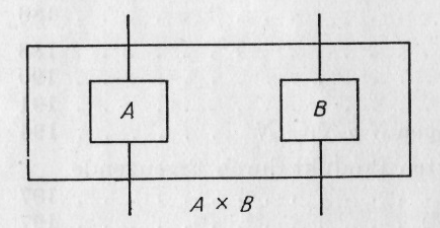
\includegraphics[]{figure1.png}
\caption{}
\label{fig:figure1}
\end{figure}

If $Z(A) = Q(B)$ we get from $A$ and $B$ a circuit $B\circ A$ by switching the $i$-th output of $A$ to the $i$-th input of $B$.

A circuit of elements of $\mathcal{U}$ is a device, which is described inductively by the preceding explanations.

If $\phi(A)$ ($\phi(B)$) is the function of circuit $A$ ($B$), then $\phi(A)\times \phi(B)$ is the function of $A\times B$, and $\phi(B)\circ \phi(A)$ for $Q(B) = Z(A)$  is the function of $B\circ A$.

The costs for the building blocks in $\mathcal{U}$ shall be defined by the function $L : \mathcal{U} \rightarrow N \cup {0}$. We define:

\[
\begin{array}{lcr}
L(A\times B) & = & L(A) + L(B), \\
L(A\circ B) & = & L(A) + L(B).
\end{array}
\]

Hereby a price is assigned to each circuit.

Now, the task is the following: Given $f : S^n \rightarrow S^m$, find a circuit $A$ with $\phi(A) = f$ and
\[
L(A) = \min_{B \in \phi^{-1}(f)} \{ L(B) \}.
\]

If $f$ does not fully map to $S^n$, but only to $R \subset S^n$, then the optimum shall be searched on $\cup_{g|R=f} \phi^{-1}(g)$. 

The task is generalized in an obvious way, if $Q(f) = Z(F) = S^n$ and $f$, as it is often the case with finite automata, is determined just by a transformation of $S^n$, 

In order to solve this problem it appears advantageous to know relations, which allow to generate from an element $A \in \phi^{-1}(f)$ all the elements from the class $\phi^{-1}(f)$.

In the first two sections of this work a theory of interconnection of automata will be developed, as already sketched out in the description of the task:

First, the topological notion of a \emph{planar} network is introduced. The binary operators "$\circ$" and "$\times$" will be explained for these networks. One obtains an algebraic structure $\mathcal{R}$, which is a category with respect to "$\circ$" and a semi-group with respect to "$\times$". $\mathcal{R}$ turns out to be a generalisation of the D-category (category with direct products), which we want to call \emph{$X$-Kategorie}.

$\mathcal{R}$ reflects the interconnection of automata, but does not reflect the possibility of different building blocks with the same number of inputs and outputs. This will be accommodated by assigning symbols of the alphabet $\mathcal{U}$ to inner points of the network, respecting the functions $Q : \mathcal{U} \rightarrow N \cup {0}$ and $Z : \mathcal{U} \rightarrow N \cup {0}$. One arrives at an $X$-Kategorie $\mathcal{F}(\mathcal{U})$, which possesses $\mathcal{U}$ as a free family of
generators. The elements of $\mathcal{F}(\mathcal{U})$ correspond to the set of circuits which may be yielded from $\mathcal{U}$. The mapping $\phi$, which assigns to each automaton its functions, becomes a functor $\phi:\mathcal{F}(\mathcal{U}) \rightarrow \mathcal{C}$, where $\mathcal{C}$ is the category of mappings of type $S^n \rightarrow S^m$. 

The introduction of the quotient category  $\mathcal{F}(\mathcal{U})/\mathcal{R}$ from $\mathcal{F}(\mathcal{U})$ to a relational system $\mathcal{R}$ forms the basis for the study of classes $\phi^{-1}(f)$. In section 3 $\phi^{-1}(f)$ will be studied for certain categories $\mathcal{F(U)}$ and distinguished functors $\phi$: We consider only families of generators $\mathcal{U}$ with $\{U, V, D\} \subset \subset \mathcal{U}$ and $Z(A) = 1$ for $A\in \mathcal{U} \setminus \{U, V, D\}$ and functors $\phi$, for which $\phi(U)$ is the mapping from $S$
to $S^{\circ}$, $\phi(V)$ the permutation of the components of $S^2$, and $\phi(D)$ the diagonalisation $S \rightarrow S^2$. Such functions are called \emph{normal}. A relational system $\mathcal{R}$ will be given with the following property: For each normal $\phi$ it holds that $\phi(F) = \phi(G)$ for $F, G \in \mathcal{F}(\mathcal{U})$, iff $F\equiv G(\mathcal{R})$. $\mathcal{F}(\mathcal{U})/\mathcal{R}$ is a $D$-category and $\mathcal{U} \setminus \{U, V, D\}$ a free family of generators of the
$D$-category.

Thus, the relational system allows to simplify the representations $F$ of a function $\phi(F)$, which are possible without the knowledge of the elements in $\mathcal{U} \setminus \{ U, V, D \}$. Figure \ref{fig:figure2} shows that there are proper simplifications in this system.

\begin{figure}
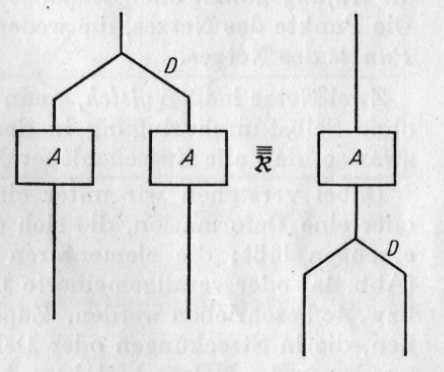
\includegraphics[]{figure2.png}
\caption{}
\label{fig:figure2}
\end{figure}

In this work we allow an arbitrary countable set for $S$, such that these results can also be of interest for computer programming. If one wants to formally simplify programs which are constructed from sub-programs, then the number of possible sub-programs renders the specific consideration of the computed function infeasible, but the rules for the transformation of programs have to be applicable uniformly for all sub-programs. Thus, that means that the allowed relations have to be the system
$\mathcal{R}$ or an equivalent system.

For an orientation on the state of the art of the theory of circuit synthesis refer to \cite{circuit-synthesis}, in relation to Streckenkpomplexen to \cite{combinatory-topology} and category theory to \cite{categories-functors} and \cite{category-theory}.
For stimulating discussions and critical remarks I want to thank J. D\"{o}rr and D. Puppe. My thanks go to the Deutsche Forschungsgemeinschaft, who has supported this study with a grant of the FRITZ-THYSSEN-foundation.

\section{The category of planar networks }
\subsection{The category $\mathcal{R}$ of planar networks}
The following topological structure is understood as a network with $n$ inputs and $m$ outputs ($n, m = 0, 1, 2...$):
A rectangle with sides $g_1, g_2$ and $h_1, h_2$ is given in the euclidean plane, where both $g_i$ and $h_i$ lie face to face to each other. $A_1 \ldots A_n$ ($B_1 \ldots B_n$) are mutually distinct points on $g_1$ ($g_2$), where the numbering of points runs from $h_1$ to $h_2$; the $A_i$ ($B_i$) divide $g_1$ ($g_2$) into equidistant parts. 
Let $A_i$ be the starting points and $B_i$ be the endpoints of precisely one line segment of an oriented, finite, planar Streckenkomplex, which lies in the euclidean plane without crossings in the rectangle \footnote{In the euclidean sense it is a matter of piecewise linear curves. }. We further demand from the Streckenkomplex that each of its line segments simply lie above $h_i$ and that the orientation of the line segments points from $g_1$ to $g_2$. Thus the case in figure \ref{fig:figure3} is
excluded.
\begin{figure}
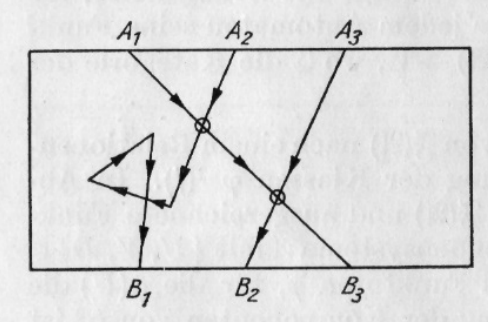
\includegraphics[]{figure3.png}
\caption{}
\label{fig:figure3}
\end{figure}

We call $g_1, g_2, h_1, h_2$ the network frame, $A_1, \ldots, A_n$ ($B_1, \ldots, B_m$) the \emph{starting points} or inputs (\emph{end points} or outputs) of the network. The points which are neither inputs nor outputs are called \emph{inner points} of the network.

Two networks are called equal, if they can be - after overlaying their frames without self-penetration in the plane - deformed into one another, in such a way that all intermediate positions are networks. 

We understand a \emph{deformation} as an \emph{elementary deformation} or a deformation, which may be generated by a chain of elementary deformations; the elementary deformations are triangular deformations (figure \ref{fig:figure4}a) or generalised triangular deformations, as shown on figure \ref{fig:figure4}b and \ref{fig:figure4}c. Further the (trivial) deformations are allowed, which are stretches of the frame or euclidean motions of the network.
\begin{figure}
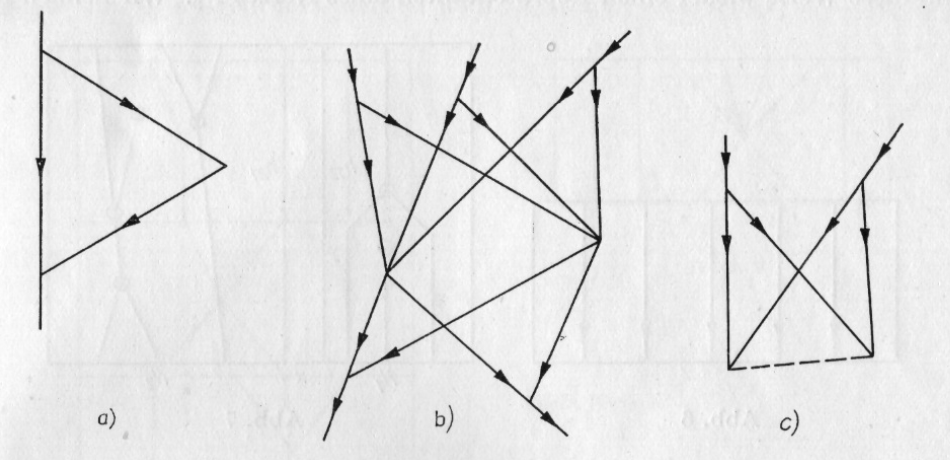
\includegraphics[]{figure4.png}
\caption{}
\label{fig:figure4}
\end{figure}

One recognises that the given equivalence definition is reflexive, symmetric and transitive, i.e. a division of the network into equivalence classes. 

From now on we call this class a network and call networks in the conventional sense, when a distinction is important, \emph{representative} of a network.

Different representatives of a network have the same number of inputs and outputs, which we denote by $Q(N)$ and $Z(N)$.

Let $N_1$ and $N_2$ be networks with $Q(N_2)=Z(N_1)$, then we declare between $N_1$ and $N_2$ a composition over representatives $N_1^{'}$ and $N_2^{'}$ from $N_1$ and $N_2$: 

We deform the frame of $N_2^{'}$ (in a trivial manner), such that we can join $N_2^{'}$ onto $N_1{'}$; i.e. we bring $g_2$ and $g_1^{'}$ to the same size and set both frames along $g_2$ and $g_1^{'}$ against each other (figure \ref{fig:figure5}). We remove $g_2 = g_1^{'}$ and the points $A_i^{'} = B_i$ and get again a network representative, that we call $N_2 \circ N_1$. One sees that the definition is independent of the choice of representatives. 

\begin{figure}
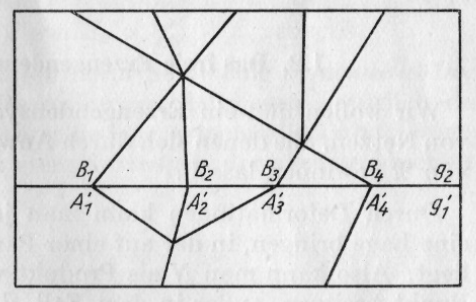
\includegraphics[]{figure5.png}
\caption{}
\label{fig:figure5}
\end{figure}

Further the following holds:

\[
\begin{array}{lcr}
Q(N_2 \circ N_1) & = & Q(N_1), \\
Z(N_2 \circ N_1) & = & Z(N_2).
\end{array}
\]

As is shown easily, the product is associative; i.e. it holds for networks $N_1, N_2, N_3$ with $Q(N_2) = Z(N_1)$ and $Q(N_3) = Z(N_2)$ that
\[ (N_3 \circ N_2) \circ N_1 = N_3 \circ (N_2 \circ N_1). \]

For each network with $Q(N) = n$ and $Z(N) = m$ there is exactly one network $E_n$ and $E_m$ with the property

\[
N\circ E_n = E_m \circ N = N;
\]

$E_n$ is a network with $n$ inputs, $n$ outputs and $n$ line segments (figure \ref{fig:figure6}). The set of networks therefore forms a category with respect to "$\circ$".

\begin{figure}
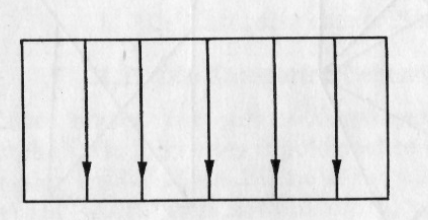
\includegraphics[]{figure6.png}
\caption{}
\label{fig:figure6}
\end{figure}

We declare a further combination of networks, namely the \emph{X-product}. Let $N_1^{'}$ and $N_2^{'}$ be representatives of the networks $N_1$ and respectively $N_2$, then we deform the frame to the same length and set them along $h_{12}$ and $h_{21}$ together (figure \ref{fig:figure7}). Subsequently we delete $h_{21}=h_{12}$ and numbering the inputs from left to right. If we take care that the input- and output-points of the structure are again equidistant, then we have again a representative
of a network $N_3$. We call $N_3$ the direct product of $N_1$ and $N_2$ and write $N_3 = N1 \times N_2$. One sees that the direct product is independent of the choice of the representative, associative, and that $E_k = E_1 \times \ldots \times E_1$ ($k$-times), and $E_0 \times N = N \times N_0 = N$ for every network $N$.

We call the set of networks with these two connections with $\mathcal{R}$. We summarize the results into

\begin{theorem}
$\mathcal{R}$ forms a category with respect to "$\circ$" and a semi-group with respect to "$\times$".
\end{theorem}

\begin{figure}
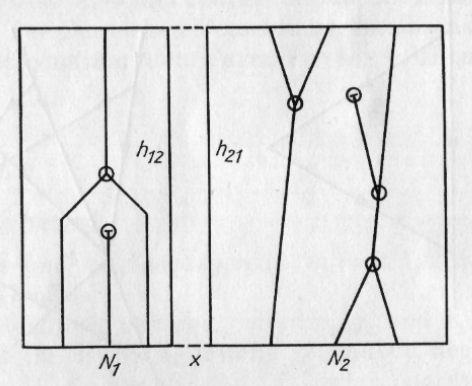
\includegraphics[]{figure7.png}
\caption{}
\label{fig:figure7}
\end{figure}

\subsection{The free family of generators of $\mathcal{R}$}

We now want to specify a family of generators for $\mathcal{R}$, i.e. the set $\mathcal{C}$ of networks, from which all networks of $\mathcal{R}$ can be obtained by application of the operations of $\mathcal{R}$.

It is possible to bring each representative of a network into a position in which at most one inner point lies on a parallel to $g_1$. Thus, $N$ may be obtained as a product of networks, which each possess one inner point, expect the case that $N$ does not possess an inner point, thus it is a unit (figure \ref{fig:figure8}).

\begin{figure}
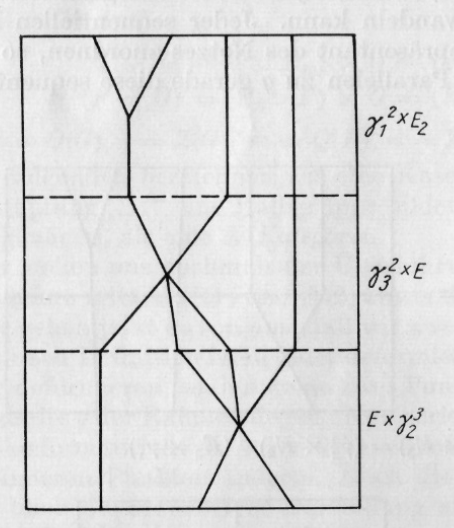
\includegraphics[]{figure8.png}
\caption{}
\label{fig:figure8}
\end{figure}

Each network $N$ with exactly one inner point can be factored into a direct product 
\[
N = E_k \times F \times E_m
\]

where $F$ contains the inner point and each line segment of $F$ possesses this point as start- and end-point (figure \ref{fig:figure9}). Potentially $k = 0$ or $m = 0$. $F$ is completely determined by the number of its inputs and outputs. If $F$ has $n$ inputs and $m$ outputs we write $\gamma_m^n$ for $F$.

\begin{figure}
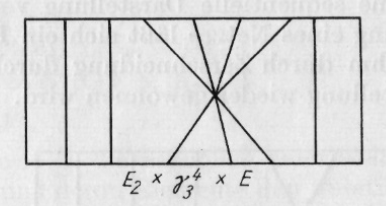
\includegraphics[]{figure9.png}
\caption{}
\label{fig:figure9}
\end{figure}

Thereby we have

\begin{theorem}
The set $\mathcal{C} = \{ \gamma_m^n | n, m = 0, 1, \ldots \}$ is a complete family of generators of $\mathcal{R}$
\end{theorem}

One recognizes further that the family of generators is minimal, since no generators can be expressed in termes of other generators. $\mathcal{C}$ is also the only minimal family of generators of $\mathcal{R}$, because no generator can be expressed through other elements of $\mathcal{R}$ other than through itself; the latter follows, because the number of inner points of a product are equal to the sum of inner points of the factors. Later (section \ref{basis-function-representation}) we will show that $\mathcal{C}$ is
a free family of generators.

The presentation of a network $N$ in this form is called a \emph{sequential presentation} of $N$. The same sequential presentations naturally define the same network, but the same network allows different sequential presentations. The next section will provide information on the different presentations of a network.

\subsection{The relations of $\mathcal{R}$}

It follows directly from the definition of the deformations that the following relations hold
\begin{equation}
\label{eq:R1}
\tag{R1}
(E_{n+k} \times \gamma_j^l) \circ (\gamma_n^m \times E_{k + l}) = (\gamma_n^m \times E_{k+j}) \circ (E_{m+k} \times \gamma_j^l) 
\end{equation}
for $k, m, n = 0, 1, 2, \ldots$ (see figure \ref{fig:figure10}).


\begin{figure}
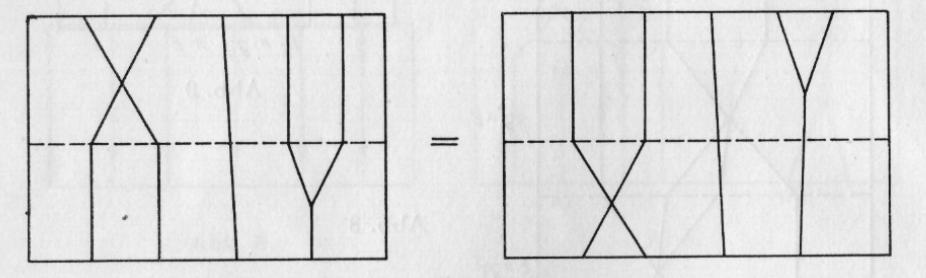
\includegraphics[]{figure10.png}
\caption{
  $(E_{3} \times \gamma_2^1) \circ (\gamma_2^2 \times E_{3}) = (\gamma_2^2 \times E_{2}) \circ (E_{3} \times \gamma_2^1)$ 
}
\label{fig:figure10}
\end{figure}

Further the following relations hold for $F, G, H \in \mathcal{R}$ with $m = Q(F), n = Z(F)$ and $Q(H)=Z(G)$
\begin{equation}
\label{eq:R2}
\tag{R2}
\left.
\begin{array}{c}
(H \circ G) \times F = (H \times F) \circ (G \times E_m) = (H \times E_n) \circ (G \times F), \\
F \times (H \circ G) = (F \times H) \circ (E_m \times G) = (E_n \times H) \circ (F \times G)
\end{array} 
\right\}
\end{equation}

(cf. figure \ref{fig:figure11}).

One sees that the relations (\ref{eq:R1}) are contained in (\ref{eq:R2}).


\begin{figure}
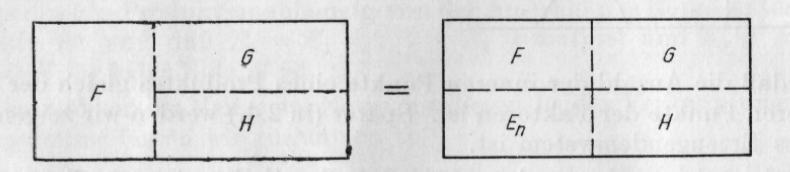
\includegraphics[]{figure11.png}
\caption{}
\label{fig:figure11}
\end{figure}

\begin{theorem}
Two presentations $H_1$ and $H_2$ of the same network in the generator family $\mathcal{C}$ under the usage of connections of $\mathcal{R}$ can be transformed via (\ref{eq:R2}) into each other.
\end{theorem}
\begin{proof}
It is apparent that every presentation can be transformed into a sequential presentation with (\ref{eq:R2}). For each sequential presentation of a network a presentation of the network may be assigned, such that exactly these sequential presentations may be recovered by cutting through parallels to $g$.
\end{proof}

Following the previous results, we may suppose that $H_1$ and $H_2$ are sequential presentations of the same network. Let $N_1^{'}$ and $N_2^{'}$ be assigned to $H_1$ and $H_2$ in the previously described manner. After defining equality $N_1^{'}$ may be deformed into $N_2^{'}$. Each step of deformation may be divided into sub-deformations such that the order of at most two points of the network is changed, because no two points in $N_1$ by construction lie on a parallel to $g$. The sequential
presentation of the network stays the same, if the order of points is not changed. If it is changed we consider the two corresponding factors of the sequential product. These shall have the form
\[
(E_t \times \gamma_n^m \times E_s) \circ (E_r \times \gamma_j^l \times E_q).
\]
Using (\ref{eq:R2})


\section{Definition of categories by a direct product through generators and defining relations}
\subsection{Representation of functions with basis functions}
\label{basis-function-representation}

\begin{thebibliography}{9}
\bibitem{zoepfe}
Artin, E., Theorie der Zöpfe. Abh. des Math. Seminars der Hamburgerischen Universit\"{a}t Bd. IV (1926).

\bibitem{circuit-synthesis}
Curtis, H. A., A New Approach to the Design of Switching Circuits. D. van Norstrand Com., Princeton 1962

\bibitem{computability}
Hermes, H., Aufz\"{a}hlbarkeit, Entscheidbarkeit, Berechenbarkeit. Springer-Verlag, Berlin-G\"{o}ttingen-Heidelberg 1961

\bibitem{categories-functors}
Puppe, D., Kategorien und Funktoren. Ausarbeitung einer Vorlesung an der Universit\"{a}t Saarbr\"{u}cken im Sommersemester 1963

\bibitem{combinatory-topology} 
Reidemeister, K., Einf\"{u}rung in die kombinatorische Topologie. Vieweg-Verlag, Braunschweig 1951

\bibitem{category-theory}
Kurosch, A. G. u. a., Zur Theorie der Kategorien. Mathematische Forschungsberichte XV. Deutscher Verlag der Wissenschaften, Berlin 1963
\end{thebibliography}

\end{document}




